\scanpage{183}
$\pi_0$

\figure{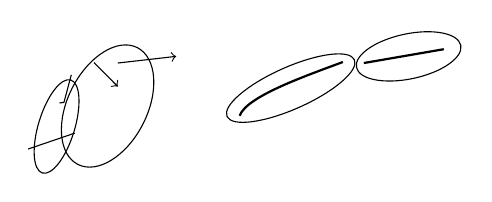
\begin{tikzpicture}[x=.72cm,y=.65cm]
\draw[thin,rotate around={-17:(.55,.65)}] (.55,.65) ellipse (.32 and .95);
\draw[thin,rotate around={-27:(1.45,1.05)}] (1.45,1.05) ellipse (.7 and 1.28);
\draw[thin] (.05,.21) -- (.87,.52);
\draw[thin] (.81,1.66) -- (.68,1.12) -- (.6,1.11);
\draw[->,thin] (1.21,1.9) -- (1.63,1.43);
\draw[thin,->] (1.63,1.89) -- (2.66,2.02);
\draw[rotate around={24:(4.68,1.4)}] (4.68,1.4) ellipse (1.23 and .41);
\draw[thick] (3.78,.86) .. controls (3.9,1.24) and (4.95,1.64) .. (5.6,1.91);
\draw[rotate around={12:(6.76,2.02)}] (6.76,2.02) ellipse (.94 and .44);
\draw[thick] (5.97,1.89) -- (7.38,2.16);
\end{tikzpicture}}

\diagram{\begin{tikzcd}[ampersand replacement=\&,column sep=1em]
F^0\arrow[r,shift left=.6ex]\arrow[r,shift right=.6ex]\& F^1\arrow[r,shift left=1.1ex]\arrow[r]\arrow[r,shift right=1.1ex]\&F^2
\end{tikzcd}}

foncteurs $(\mathrm{Ens})\to(\mathrm{Ens})$

objet simplicial de $\underline{\operatorname{Hom}}(\mathrm{Ens},\mathrm{Ens})$

Permet en principe de définir des $\pi_0,\pi_1$

$\pi_0(F)$, $F\in\underline{\operatorname{Hom}}(\mathrm{Ens},\mathrm{Ens})$, $F$

\[
F(I)\underset{?}{\simeq}C(K,I)\qquad K\ \text{espace top \uline{tot. discontinu}}
\]
[deux pts sont séparés par un ens : à la fois ouvert et fermé]

\uline{Cond néc} a) $F$ commute aux \deleted{\unsure{produits}} $\varprojlim$ finies i.e. $F$ \uline{exact à gauche} [donc $F$ transforme mon. en mon]

b) $F(\bigcap I_\alpha)=\bigcap_\alpha F(I_\alpha)$ pour \deleted{\unsure{(tous)|(toute)}} famille filtrante de sous-ens. de $I$

Ces conditions équivalent à : \uline{$F$ strictement proreprésentable} par un système projectif strict $(\pi_{0\,i})_i$ \deleted{\unsure{de}} d'ensemble.

Il faut de plus

c) $\deleted{\unsure{\pi_0=|\text{Alors}}}\varprojlim\pi_{0\,i}\longrightarrow\pi_{0\,i}$ est \uline{surjectif} pour $\forall\,i$

Ces conditions sont \uline{néc} et suffisantes, et on pourra prendre $K=\varprojlim\pi_{0\,i}$, avec la topologie limite inverse des top. discrètes. \uline{NB} \unsure{Si} $F$ est donné dans la forme $C(L,I)$, $L$ esp. top., alors $\pi_0(L)\longrightarrow K$. Si $L$ est \inserted{(quasi)} compact, cet hom est un isomorphisme ; \uline{en général}, ce n'est ni injectif, ni surjectif,

\margin{Bourb. Topologie \unsure{II|2} p. 232, prop. 6}

% archive sheet number: 182
